%!TEX program = xelatex
% 代码前 \vspace{-0.8cm}
% 图片画布18cm,设置宽度width=0.9\textwidth

\documentclass[listof = totoc]{article}
% 加入listof = totoc以解决代码无法列入目录

\usepackage{amsmath}
\usepackage{supertabular}

% 页面------------------------------------------------------------------
\usepackage[centering,paperwidth=180mm,paperheight=230mm,%
body={390pt,530pt},marginparsep=10pt,marginpar=50pt]{geometry}
% body 137mmx186mm

% 页眉页脚
\usepackage{fancyhdr}

% 图片------------------------------------------------------------------
\usepackage{graphicx}    

% 符号------------------------------------------------------------------
\usepackage{trfsigns}
\usepackage{mathabx}

% 颜色------------------------------------------------------------------
\usepackage{color}
\definecolor{commentcolor}{RGB}{34,139,34}
\definecolor{codecolor}{RGB}{34,139,34}
\definecolor{mycolor}{RGB}{129,0,0}

% 背景------------------------------------------------------------------
\usepackage{framed}
\definecolor{shadecolor}{gray}{0.92}
% 用于shaded的背景

% 链接------------------------------------------------------------------
\usepackage{url}
\usepackage{hyperref}
\hypersetup{pdftitle = {Chen's MATLAB Learning},
    colorlinks = true,
    pdfborder = 0 0 0,
    linkcolor = mycolor,
    urlcolor = mycolor,
    breaklinks = false}

% 代码------------------------------------------------------------------
\usepackage{mcode}
\usepackage{listings}
\lstset{numbers = none,                       % 代码行号
  % numberstyle = \scriptsize,
  % frameround = fttt,                          
  frame = lines,                              % 边框 trBL single
  backgroundcolor = \color{white},            % 背景颜色
  language = Matlab,
  keywordstyle = \color{blue},                % 关键词颜色
  commentstyle = \color{commentcolor},        % 注释颜色
  basicstyle = \linespread{1}\fontspec{Consolas}\small,  % 代码字体
  emph={warning,pcode},                       % 自定义关键词
  emphstyle=\color{blue},                     % 自定义关键词颜色
  texcl = true}
% 在对应的设置中加入 nolol=true 以不列入目录中
% 只要不加入caption就不会录入目录

% 表格------------------------------------------------------------------
\usepackage{multirow}
\usepackage{arydshln}
\usepackage{multicol}
\usepackage[hang, small,labelfont=bf,up,textfont=it,up]{caption}
\usepackage{booktabs}
\usepackage{float}

% 段落------------------------------------------------------------------
\usepackage{indentfirst}
\setlength{\parindent}{2em}   % 段首缩进
\setlength{\parskip}{2.0pt}   % 段间距
\linespread{1.3}              % 行间距

% 字体------------------------------------------------------------------
\usepackage{xeCJK}
\setmainfont{Times New Roman}
\setCJKmainfont[BoldFont=SimHei]{SimSun}
\setCJKfamilyfont{kai}{KaiTi}
\newcommand{\kai}{\CJKfamily{kai}}

% 定义注意事项notation------------------------------------------------------------------
\usepackage{amsthm}
\theoremstyle{remark}
\newtheorem{nota}{Note}[section]
\newcommand{\notation}[1]{\nota{\kai #1}}

% item
\usepackage{mdwlist}          % item 压缩
\usepackage{enumitem}
\newcommand\begindot{\begin{itemize}
[itemsep=2pt plus 2pt minus 2pt,%
topsep=3pt plus 2pt minus 2pt,%
parsep=0pt plus 2pt minus 2pt]}
\newcommand\myenddot{\end{itemize}}

% 其他------------------------------------------------------------------
% \renewcommand{\today}{\the\year-\the\month-\the\day}

%----------------------------------------------------------------------------------------
%	TITLE PAGE
%----------------------------------------------------------------------------------------
% http://www.latextemplates.com/cat/title-pages
\newcommand*{\titleCover}{\begingroup % Create the command for including the title page in the document
\hbox{ % Horizontal box
\hspace*{0.15\textwidth} % Whitespace to the left of the title page
\rule{1pt}{\textheight} % Vertical line
\hspace*{0.05\textwidth} % Whitespace between the vertical line and title page text
\parbox[b]{0.75\textwidth}{ % Paragraph box which restricts text to less than the width of the page

{\noindent\Huge\bfseries MATLAB \\[0.5\baselineskip] 学习笔记 0.1.1v}\\[2\baselineskip] % Title
{\large \textit{MATLAB学习之路:功能与效率}}\\[4\baselineskip] % Tagline or further description
{\Large \textsc{陈磊}} % Author name

\vspace{0.5\textheight} % Whitespace between the title block and the publisher
{\noindent \today\\
\textit{email chenlei.here@gmail.com\\
blog {\href{http://herechen.github.io}{herechen.github.io}}\\source {\href{https://github.com/HereChen/TheWayMATLABLearning}{https://github.com/HereChen/TheWayMATLABLearning}} }}\\
[0.0\baselineskip] % Publisher and logo
}}
\endgroup}

% \title{MATLAB学习笔记}
% \author{陈磊\\chenlei.here@gmail.com}
% \date{\today}


\begin{document}

% \renewcommand{\abstractname}{摘要}
% \renewcommand{\contentsname}{目录}
% \renewcommand{\tablename}{表格}
\renewcommand{\lstlistlistingname}{List of Examples}
\renewcommand{\lstlistingname}{Example}
\newcommand\BookTitle{MATLAB学习笔记}

% \pagestyle{fancy}
% \fancyhead[L]{{\normalfont\small\rmfamily\nouppercase{\leftmark}}}
% \fancyhead[C]{{\normalfont\small\rmfamily\nouppercase{\rightmark}}}
% \fancyhead[R]{{\thepage}}
% \fancyfoot[L]{{\small\kai\BookTitle}}
% \fancyfoot[C]{}
% \fancyfoot[R]{{\href{http://herechen.github.io}{herechen.github.io}}}

\thispagestyle{empty}
\titleCover
% \maketitle
% \begin{abstract}
这份文档于2013年的夏天开始撰写。不同于开始,后来我是这样打算的,以简洁的方式呈现自己所学的MATLAB知识。一则温故知新,二则留存一份历史,如是而已。\par
文中写作上既不全面描述,也不过于细致描述,简单描述的目的在于“知”,知道一些功能,知道一些技巧,然后可以探究。
% \end{abstract}

\begin{multicols}{2}
\tableofcontents
\listoftables
\listoffigures
\lstlistoflistings
\end{multicols}

\graphicspath{{diagrams/}}

\section{学途伊始}
最开始学习MATLAB是从脚本开始的,写一段然后就选中代码按F9这种.后来逐渐需
要把一些通用或常用的脚本写成函数,需要的时候一句话就可以调用了.这大概也
就是整体上我的学途历程了.\par
再往后,就开始考虑效率,接触一些方便好用的功能,考虑算法设计和
MATLAB编程特性的结合,如何去调试程序等等.\par
那么,我们以脚本和函数开始.

\subsection{窗口}
MATLAB有几个基本的窗口: Command Window用于输出结果以及执行命令之用; Editor
则作为编辑代码之用;在Workspace可以看到当前保存的变量; Command History保
存了执行过的命令的历史记录; Current Folder是当前目录,方便了管理多个文件编
辑的需求.

\subsection{脚本}
也不知道如何解释脚本(Script)这个词才好.在MATLAB里面Ctrl+N新建一个后缀
为m的文件,也就是通常说的M-file.写入要实现的东西,选中要执行的代码然后按F9就可
以在Command窗口查看结果.比如给出的例子就包含了注释、一个输出语句以及一
个矩阵的赋值.

\begin{lstlisting}[caption=第一个脚本]
  disp('Hello MATLAB') % 我是注释,前面一条语句是输出
  A = [1 2; 3 4];      % 对A赋值,A是一个矩阵,语句不加分号执行会直接输出
\end{lstlisting}

\subsection{函数}
把常用到的功能或者具有一定功能的单独拿出来,写成一个函数,在需要的时候直
接调用.这一方便避免的代码的重复书写,又方便了程序的调试.函数不能在当前
文件执行,需要通过调用的形式来执行.比如下面的这个函数保存为文件之后,可
以直接在Command窗口调用.

\begin{lstlisting}[caption = 第一个函数]
  function sm = twonosum(no1,no2)
  % 两个数之和
  sm = no1 + no2;
  end
\end{lstlisting}

\begindot
  \item 保存时需要和函数名一致,上面的例子应保存为twonosum.m;
  \item Command窗口或脚本调用格式为\mcode{var1 = twonosum(var2,
      var3)};
  \item 文件twonosum.m所在路径需要添加,这在文中的路径设置中提到;
\myenddot

\notation{最后的\mcode{end}并非是必须的,可以删除.}


\subsection{一个实例}
通过牛顿法法解非线性方程来展示一个函数的书写,同时也展示了如何调用.在这
里,实现的内容并不是关键,关键在于展示一种写作风格和实现的方法.

\paragraph{牛顿法算法}
用牛顿法解方程 \(f(x) = 0\),即用牛顿迭代式通过迭代得到近似解.牛顿法迭代式为
\[
    x_{k+1} = x_k - \frac{f(x_k)}{f^{\prime}(x_k)}.
\]
牛顿法的几本算法如下,这是后面的实现的框架.      
\begin{center}
\begin{supertabular}{l}
        \hline
        \bf{input} \(x_0,M,\delta,\varepsilon \) \\
        \(v\leftarrow f(x_0)\) \\
        \bf{output} \(0,x_0,v\) \\
        \bf{if} \(|v|<\varepsilon\) \bf{then stop} \\
        \bf{for} \(k=1\) \bf{to} \(M\) \bf{do} \\
        \qquad \(x_1\leftarrow x_0-v/f^{\prime}(x_0)\) \\
        \qquad \(v\leftarrow f(x_1)\) \\
        \qquad \bf{output} \(k,x_1,v\) \\
        \qquad \bf{if} \(|x_1-x_0|<\delta \) \bf{or} \(|v|\leftarrow \varepsilon\) \bf{then stop} \\
        \qquad \(x_0\leftarrow x_1\) \\
        \bf{end do} \\
        \hline
\end{supertabular}
\end{center}

\begin{lstlisting}[caption = 牛顿法解非线性方程]
function root = newton(f, df, x0, maxiter, tol)
%NEWTON Newton's method for nonlinear equations.
%
%   NEWTON's method: x(k+1) = x(k) - f(x(k))/f'(x(k)).
%
%   Inputs
%   f       - nonlinear equation.
%   df      - derivative of f(x).
%   x0      - initial value.
%   maxiter - maximum iterated times.
%   tol     - precision.
%
%   Outputs
%   root    - root of f(x) = 0.

%   Last Reversion: 2013/11/20  10:56:48

% 初始化,默认参数设置
if nargin < 5, tol = eps; end
if nargin < 4, maxiter = 50; end

x_old    = x0;
x_iter   = x0 + 1;
times    = 0;


IfTrue
% 输出初值信息
if true_sig
        fprintf(' k      iter\n');
        fprintf('-------+-------------\n');
        fprintf('%3.0f    | %.7f\n', 0, x_old);
end


% 通过判断是否满足条件作循环
tic
while true_sig
    x_iter = x_old - f(x_old)/df(x_old);
    times = times + 1;
    IfTrue
    x_old = x_iter;
        fprintf('%3.0f    | %.10f\n', times, x_old);
end
time = toc;
% tic开始计时,toc 结束计时

% 输出迭代次数和迭代时间
fprintf('\nIterated times is %g.\n', times);
fprintf('Elapsed time is %g seconds.\n', time);


% 输出参数,取最后一个迭代值
root = x_iter;


% 子函数,用以计算循环条件的逻辑值
    function IfTrue
        if times == 0
            true_sig = (times < maxiter) ...
                   && (abs(x_old - x_iter) > tol) ...
                   && (abs(f(x_old)) > tol);
        else
            true_sig = (times < maxiter) ...
                   && (abs(x_old - x_iter) > tol) ...
                   && (abs(f(x_iter)) > tol);
        end
    end

end
\end{lstlisting}        

牛顿法实现的调用的示例如下,这个例子用于求解2的平方根.

\vspace{-0.5cm}
\begin{lstlisting}
  f = @(x)x^2 - 2;          % 函数,匿名函数
  df = @(x)2*x;             % 导数
  x0 = 3;                   % 迭代初值
  root = newton(f, df, x0); % 未输入的参数取默认参数
\end{lstlisting}

这个实例涉及到函数、子函数、计时、逻辑运算、默认参数设置、匿名函数,以及模仿
MATLAB内置函数写函数注释.最后再给出了运行示例,算是一个完整的算法实现.实
际上,未必都要如此编写程序,根据个人需求,达到目的即可,这里只作为一个范例.
\section{一些功能}

\subsection{快捷键}

\begin{center}
% Table generated by Excel2LaTeX from sheet 'Sheet1'
\begin{table}[htbp!]
  \centering
  \caption{快捷键}
    \begin{tabular}{ll|ll}
    \toprule
    \multicolumn{1}{c}{功能}    & \multicolumn{1}{c}{快捷键}   & \multicolumn{1}{c}{功能}    & \multicolumn{1}{c}{快捷键}\\
    \midrule
    注释          & Ctrl + R              & 切换到Command Window   & Ctrl + 0  \\
    自动排版      & Ctrl + I              & 切换到Command History  & Ctrl + 1 \\
    取消注释      & Ctrl + T              & 切换到 Current Folder  & Ctrl + 2  \\
    向右缩进      & Ctrl + [              & 切换到Workspace        & Ctrl + 3 \\
    向左缩进      & Ctrl + ]              & 切换到Editor           & Ctrl + Shift + 0 \\
    执行当前单元  & Shift + Ctrl + Enter  & Editor之间的切换       & Ctrl + PgDn/PgUp \\
    终止程序      & Ctrl + C              & 添加函数               & Ctrl + J \\
    上一个单元    & Ctrl + Down           & 下一个单元             & Ctrl + Up \\
    \bottomrule
    \end{tabular}%
  % \label{tab:addlabel}%
\end{table}%
\end{center}



\subsection{MATLAB启动}
这里不描述通常的点击图标启动.有这样两种启动方式:
\begindot
  \item \mcode{matlab},完全启动,即正常的启动;
  \item \mcode{matlab -nojvm},只启动Command窗口,这将禁用与java相关的功能,启动速度较快.
\myenddot
在Windows中,可以命令方式来启动,即在cmd或 \mcode{Ctrl+R} 调出的“运行”中执行,对应的命令在其后已经给出.命令启动有个前提, MATLAB的可执行程序路径已经在环境变量中.\par

\begin{figure}[htbp]
  \centering
  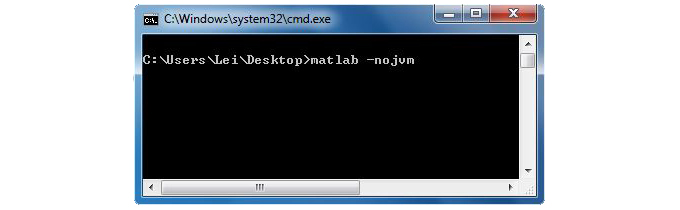
\includegraphics[width=0.9\textwidth]{startmatlab1.jpg}
\end{figure}

\begin{figure}[htbp]
  \centering
  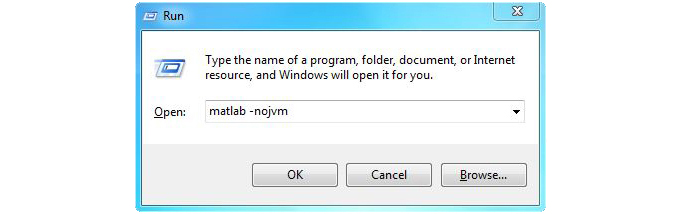
\includegraphics[width=0.9\textwidth]{startmatlab2.jpg}
  \caption{MATLAB “no java” 启动}
\end{figure}

在图中直接输入以 \mcode{matlab} 可实现完全启动.若是期望轻量级编程,可以“no java”方式启动,并配合其他编辑器(比如Sublime Text),可以实现脚本或函数的编辑及执行.对两种方式做个对比:

\begindot
  \item 完全启动,速度慢,功能齐全,占用内存大(相对);
  \item “no java”启动,速度快,功能少一部分,占用内存小.
\myenddot

\notation{MATLAB环境变量的设置.假设MATLAB安装在C:$\backslash$MATLAB目录下,那么, matlab.exe应该在C:$\backslash$MATLAB$\backslash$bin目录下.接着设置环境变量,电脑属性$\rightarrow$高级系统设置$\rightarrow$环境变量$\rightarrow$用户变量下选中PATH并点击编辑按钮$\rightarrow$添加C:$\backslash$MATLAB$\backslash$bin(在最后加入分号添加)$\rightarrow$一路保存退出}.


\subsection{路径设置}
设置路径的方法:
\begindot
\item 鼠标点击实现. Home$\rightarrow$set path. Add Folder...只添加选定文件夹的路径, Add with Subfolders...添加指定文件夹及其所有子文件夹路径.

  \begin{figure}[htbp]
    \centering
    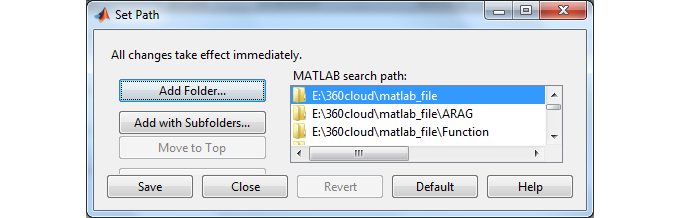
\includegraphics[width=0.9\textwidth]{setpath.png}
    \caption{添加路径}
  \end{figure}

\item 通过命令添加,比如:

\vspace{-0.8cm}
\begin{lstlisting}[caption = 添加路径]
  addpath('D:\matlab_file')
\end{lstlisting}

\item 直接通过路径文件设置.

\vspace{-0.4cm}
\begin{lstlisting}
  >> which pathdef
  C:\Program\MATLAB\R2013a\toolbox\local\pathdef.m
  >> edit('C:\Program\MATLAB\R2013a\toolbox\local\pathdef.m')
\end{lstlisting}

\item 设置工作目录. MATLAB默认的工作目录可以通过输入 \mcode{userpath} 来查看,更改则通过 \mcode{userpath(mypath)} 来实现,其中 \mcode{mypath} 是自定义的路径字符串.设置工作目录的意义在于,将需要的文件放在放在工作目录,就无需额外添加路径了.

\myenddot

添加路径的意义在于,这使得我们期待调用的脚本、函数或资源等能够被找到.

\notation{如果路径中包含空格,用 \mcode{' '} 来表示空格,即两个单引号,中间包含一个空格.}



\subsection{startup}
startup.m是在MATLAB启动时就执行的脚本.若是需要它,我们需要做三件事情:
\begindot
  \item 新建startup.m;
  \item 确保startup.m所在文件夹的路径已经添加;
  \item 编辑需要MATLAB启动就执行的内容.
\myenddot

\vspace{-0.8cm}
\begin{lstlisting}[caption = 我的startup.m]
  clc;                    % 清除Command窗口显示的内容
  cd D:\matlabfile;       % 定位到matlabfile文件夹
  addpath(genpath(pwd));  % 将当前文件夹的所有文件夹及子文件夹添加到路径中
  % pwd为获得当前文件夹路径,即D:$\backslash$matlabfile
\end{lstlisting}
这段代码执行3个命令,主要目的还是在于进入到我的工作目录,并添加可能的新的路径(因而用了 \mcode{genpath}).



\subsection{计时器}
\mcode{tic} 为计时开始, \mcode{toc} 为计时结束.通常用以查看代码/算法执行的时间.

\vspace{-0.8cm}
\begin{lstlisting}[caption = 计时1]
  tic
  disp('Time recorder...');
  toc
\end{lstlisting}

\vspace{-0.8cm}
\begin{lstlisting}[caption=计时2]
  t1 = tic;
  disp('Time recorder...');
  toc(t1)
\end{lstlisting}

\vspace{-0.8cm}
\begin{lstlisting}
  Time recorder...
  Elapsed time is 0.007663 seconds.
\end{lstlisting}

两个例子单独的执行效果如上.在使用时可以注意以下几点:
\begindot
  \item 若是不需要输出时间,在 \mcode{toc} 后加分号即可;
  \item 若需要保存记录的时间,可用变量存储,比如 \mcode{usedtime = toc} 或 \mcode{usedtime = toc(t1)} .
  \item 计时方案2适合有多个计时需求的应用.
\myenddot

\notation{另一种计时 \mcode{etime} ,但这并不是推荐的方式, \mcode{help etime} 查看.}



\subsection{代码单元}
\mcode{\%} 是注释, \mcode{\%\%} 则是一个单元(同时作为注释). 

\vspace{-0.8cm}
\begin{lstlisting}[caption=代码单元]
  %\% display 1
  disp('the first cell.');

  %\% display 2
  disp('the second cell.');
  % 两个百分号与注释之间有空格.
\end{lstlisting}

代码单元可在不选中代码的情况下,可以快捷键 \mcode{Ctrl+Shift+Enter} 连续执行.并还有以下好处:
\begindot
  \item 一个单元一个单元的执行,方便检错/调试;
  \item 方便查看过程数据;
  \item 把具有特定功能的一段代码作为一个单元,使得代码结构清晰.
\myenddot



\subsection{断点调试}
这里是针对function,通过设置断点找出错误所在,亦或了解代码执行过程.在需要暂停的一行或多行前用鼠标点击设置断点.

\begin{figure}[htbp]
  \centering
  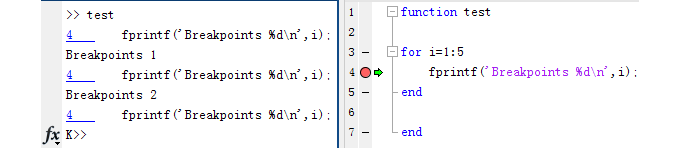
\includegraphics[width=0.9\textwidth]{breakpoint1.png}
\end{figure}

\begin{figure}[htbp]
  \centering
  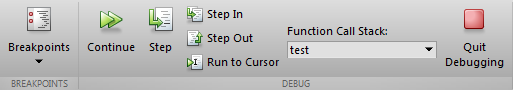
\includegraphics[width=0.9\textwidth]{breakpoint3.png}
  \caption{断点调试}
\end{figure}

相对于通过执行选中代码段来调试,这种方式更加便捷,并且适合批量操作.断点调试常用的两个快捷键:
\begindot
  \item \mcode{F5}, 继续执行;
  \item \mcode{Shift+F5}, 停止继续执行(Quit Debugging).
\myenddot



\subsection{代码发布}
 代码发布,就功能而言,即可用其他文档格式展现代码.发布的格式有多种可选,比如: latex、html、doc、ppt等等.发布方式:
 \begindot
  \item 在菜单栏Publish下设置和发布;
  \item 通过函数 \mcode{publish} 发布,查看 \mcode{help publish}.比如将test.m发布为pdf.

  \vspace{-0.8cm}
  \begin{lstlisting}[caption = 代码发布]
    publish('test.m','pdf');
  \end{lstlisting}

\myenddot

\begin{figure}[htbp]
  \centering
  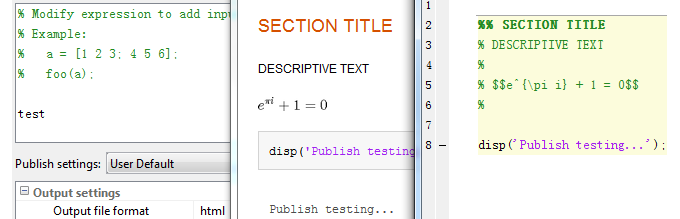
\includegraphics[width=0.9\textwidth]{publish.png}
  \caption{代码发布}
\end{figure}

发布代码的同时,结果也会一同发布,这包括输出和图像等.代码发布还有这样一些细节:
\begindot
  \item 添加章节,使代码更加直观.这可以通过代码单元来实现;
  \item 注释设置,一则可以设置字体,二则可以设置列表(list);
  \item 添加其他元素,比如:图片、公式、超链接.
\myenddot

\notation{就我当前所用版本,要发布含数学公式的建议用\LaTeX,其他几种公式转换为图片发布,效果并不好.或可用其他方式弥补也是可以的(比如先发布为\LaTeX,再生成pdf).也许,这仅仅是因为对\LaTeX的钟爱.}



\subsection{代码保护}
代码保护(protect function)从功能上来理解,有两点:
\begindot
  \item 代码加密(用这种方式生成的文件是被加密的),同时又能像其他文件一样调用;
  \item 预解析文件,直接调用解析过的文件,可以提高执行速度.
\myenddot
首先,通过 \mcode{pcode} 将m文件解析为p后缀文件;然后直接调用该文件.这里给出了针对单个文件的例子,但也可一次解析多个文件.

  \vspace{-0.8cm}
  \begin{lstlisting}[caption = 代码保护]
    pcode filename.m
  \end{lstlisting}

\notation{生成解析文件后,路径下就有两个同名,但是后缀不同的文件.对m文件修改后需要重新解析,不然,会调用较新的m文件,而不是p文件.另外,"解析"一词在这里更多的是指 \mcode{pcode} 的函数作用.}



\subsection{应用发布}
 应用发布是指把脚本或者函数编译成可执行的exe文件.应用发布包含两个步骤:

 \begindot
  \item \mcode{mbuild -setup} 选择和配置编译器;
  \item \mcode{mcc -m myfile.m} 将脚本编译成可执行文件.
 \myenddot

注意上面命令之间的空格.编译得到的同名exe文件在MATLAB安装目录的bin文件夹下,或者在所编译文件所在的文件夹下.

\subsection{警告和错误}
在编写程序时,会用一些输出来标识警告或者错误,以下是针对这个问题的方法.

\vspace{-0.8cm}
\begin{lstlisting}[caption = 红色字符串输出]
  fprintf(2,'edit your text here.');
\end{lstlisting}


\vspace{-0.8cm}
\begin{lstlisting}[caption = 警告输出]
  warning('edit your text here.')};
\end{lstlisting}

\vspace{-0.8cm}
\begin{lstlisting}[caption = 错误输出]
  error('edit your text here.')};
\end{lstlisting}

\notation{\mcode{warning} 和 \mcode{error} 可以像 \mcode{fprintf} 一样输出字符串或者数值.例如: \\
\mcode{str = 'I am a string'; warning('\%s',str)}}
\section{一些函数}

\paragraph{help} 查看帮助文档.比如:\mcode{help size}.
\paragraph{prod} 向量元素连乘,或矩阵元素的列元素连乘
\paragraph{eval}
\paragraph{pause} 暂停,暂停5秒,即\mcode{pause(5)}.
\paragraph{nnz} 零元素的个数,由此可以获得其他元素的个数(通过减法)
\paragraph{xlsread xlswrite}
\paragraph{clc} 清屏,清除Command窗口显示内容.
\paragraph{clear} 清除变量,清楚工作空间存储的变量.其后加变量名可以只清
除指定变量,比如:\mcode{clear vari}.
\paragraph{pack} 整理内存.
\paragraph{peaks} 画出一个特殊的图形来...
\paragraph{logo} MATLAB的标志.
\paragraph{version} 获得MATLAB的版本号.
\paragraph{ver} 获得MATLAB各组件的版本号.
\paragraph{load} 从硬盘加载数据.
\paragraph{save} 保存工作空间变量.
\paragraph{diary} 保存Command屏幕输出,由于屏幕输出延时,可能并没有保
存数据,因此有两个方案来应对;其一,加入pause;其二,判断是否已保存数
据,直到有数据才执行diary off.
\paragraph{exit} 退出MATLAB.
\paragraph{which} 查看函数的文件路径.比如:\mcode{which fmincon}.
\paragraph{whos} 查看当前工作空间变量的属性.查看某个变量的属性这添加变
量名作为参数,比如:\mcode{whos var} 指查看 \mcode{var} 变量的属性.
\section{一些技巧}

这里所指技巧具有专题性的意义,是面向解决方案的,而不是面向功能的讲解。





\subsection{内存溢出及解决方案}

\paragraph{内存溢出}所谓内存溢出,也就是计算时出现的 Out of memoery.

\begin{figure}[htbp]
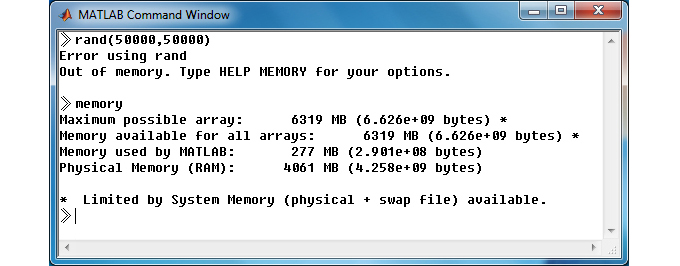
\includegraphics[width=0.6\textwidth]{memoryout}
\caption{内存溢出和内存查看}
\end{figure}

\vspace{-0.8cm}
\lstinputlisting[language=matlab, caption={生成随机矩阵测试内存溢出}]{secSkillsSome/rand-matrix.m}

\notation{逐渐增大或减小维数,这样可以测试设备能存储最大矩阵的维数。}


\paragraph{内存溢出解决} 简而言之,开源节流。

\begindot
  \item 开源方法
    \begin{itemize*}
    \item 增加RAM。买个大点的内存条装上;
    \item 以“no java”方式启动MATLAB。(这是在节MATLAB的流,开程序执行的源)
    \end{itemize*}
  \item 节流方法
    \begin{itemize*}
    \item 数据本地存储。将数据存储到本地,需要时再导入;
    \item 使用已有的变量,即时删除临时变量(不再需要的变量);
    \item 以函数封装。将程序中某几部分的代码封装为 function 调用,function 调用只输出最后需要的数据,其间的临时变量在每次调用完 function 之后都会自动删除。
    \end{itemize*}
\myenddot





\subsection{自定义函数帮助}

在MATLAB中可以用输入help加函数名来获得获悉使用方法及例子。我们期望对自己编写的函数也实现这样的功能,那么有两个关键点,一是参照MATLAB的内置函数注释格式写好注释(或者参照下面的示例),二是确保此函数路径已经添加。接下来就可以通过 \mcode{help myfunction} 这样的形式来查看了。

\vspace{-0.8cm}
\lstinputlisting[language=matlab, caption={自定义帮助}]{secSkillsSome/define-help-comment.m}





\subsection{图像导出}

除了一般的截图方法,有这样几种方法。

\begindot
  \item \mcode{print('-dpdf',pdf_name);},生成图像为pdf格式。
  \item 直接设置导出, File - Export Setup - Export,通过 Rendering - Resolution 可以设置图像质量。
  \item \mcode{saveas(gcf, 'output', 'jpg')},导出当前figure为名为output的jpg格式图像。
\myenddot





\subsection{公式打印}
MATLAB 支持 \LaTeX 的公式输出,在两个地方可能用到公式输出。

\begindot
  \item 图片上的公式。
  \item 代码发布注释中的公式。
\myenddot

\vspace{-0.8cm}
\lstinputlisting[language=matlab, caption={图像中的公式输出}]{secSkillsSome/math-in-figure.m}





\subsection{重复向量以构造矩阵}

首先解释一下什么是向量重复构造矩阵(并非是一个专业术语),比如有一个向量 \mcode{[1 2 3]},现在我打算将它构造成 \mcode{[1 2 3; 1 2 3; 1 2 3]},这就是此小节要解决的内容。

\vspace{-0.8cm}
\lstinputlisting[language=matlab, caption={重复向量以构造矩阵}]{secSkillsSome/repeat-matrix.m}

\vspace{-0.8cm}
\lstinputlisting[language=matlab, nolol]{secSkillsSome/repeat-matrix-result.m}


实际上,\mcode{repmat} 用到了第三种,在其源码中可以看的到,但它更加通用。如果是数值,首推第三者。
 \mcode{repmat} 的源码可以通过 \mcode{which repmat} 查看其位置。另外需要提及,测试时每段前面当加 \mcode{clear},这是要消除由于内存的原因影响后面程序的执行效率。\par

还有一种方式,这种方式可以列重复挨着:

\vspace{-0.4cm}
\lstinputlisting[language=matlab, nolol]{secSkillsSome/repeat-matrix-2.m}

\notation{可以考虑用上面的某种方法用向量重复来构造三维的矩阵。}
\section{高效编程}

\subsection{profile}
 通过 profile 这个工具来查看执行程序中占用时间比例较大的部分,并作有针对性的优化. profile on,profile viewer % go on

\subsection{数据类型}
 double,cell

\subsection{预分配内存}
 为矩阵(或向量)预分配内存,并尽量避免改变矩阵的大小.为什么预分配内存呢?实际上,申请新的内存本身就是一种耗费.每当申请需要新的内存存储变量时,MATLAB 都会先查找是否有足够并且逻辑上是连续的内存空间来存储(若没有则会内存溢出,无法继续执行程序). 对于矩阵,每次对它添加元素时,其所占内存就在改变,这种改变在地址上的本质是,它不是在原有的基础上添加,而是找到一块合适的地址之后,存储到新的空间上,并删除原来空间上的数据.

  \vspace{-0.8cm}
  \begin{lstlisting}[caption = 预分配内存]
    n = 1e+7;
    % 未初始化赋值
    tic
    for i=1:n
        a(i) = i;
    end
    toc

    % 初始化后赋值
    tic
    b = zeros(1,n,'double');
    for i=1:n
        b(i) = i;
    end
    toc
  \end{lstlisting}

  \vspace{-0.8cm}
  \begin{lstlisting}
    Elapsed time is 4.193847 seconds.
    Elapsed time is 0.177962 seconds.
  \end{lstlisting}

\subsection{临时变量}
 尽量少使用临时变量,毕竟申请内存是一件耗费的事情.

\subsection{MATLAB 建议}
 根据 MATLAB 建议编写程序(有时候编程会出现黄色下划线). 当然,不是任何时候都根据它的建议来,有时候我们也发现 MATLAB 会“多管闲事”.

\subsection{矩阵存储方式}
 矩阵的存储方式以列优先存储,即我们在计算时尽量采用列优先的方式.\\% 此处加一例,两重for 循环的计算.

  \vspace{-0.8cm}
  \begin{lstlisting}[caption = 矩阵存储的方式]
    n = 5*1e+3;
    A = rand(n , n);
    B = zeros(n , n);

    % 以行存取
    tic
    for i = 1:n
        B(i , :) = A(i , :);
    end
    toc

    % 以列存取
    tic
    for i = 1:n
        B(: , i) = A(: , i);
    end
    toc
  \end{lstlisting}

  \vspace{-0.8cm}
  \begin{lstlisting}
    Elapsed time is 0.945340 seconds.
    Elapsed time is 0.150333 seconds.
  \end{lstlisting}

\subsection{函数类型}
 不同函数类型的执行效率并一样,在此仅以符号函数和匿名函数作为对比对象.

  \vspace{-0.8cm}
  \begin{lstlisting}[caption = 函数类型]
    % 符号函数
    syms fun1(x);
    fun1(x) = x^3 + x^2 + x +1;
    tic
    fun1(5);
    toc

    % 匿名函数
    fun2 = @(x)x^3 + x^2 + x +1;
    tic
    fun2(5);
    toc
  \end{lstlisting}

  \vspace{-0.8cm}
  \begin{lstlisting}
    Elapsed time is 0.006139 seconds.
    Elapsed time is 0.000074 seconds.
  \end{lstlisting}

\subsection{并行计算}
 所谓并行计算,则是让多个工作同时进行以节省时间,而这些工作之间并不存在数据上的依赖.matlabpool parfor

\subsection{混合编程}
 ....尚未实践.
\section{额外兴趣}

\subsection{拍照}
用MATLAB调用硬件拍照简单示例(确保有可用的摄像头,并一段一段执行):

  \vspace{-0.8cm}
  \begin{lstlisting}[caption = 拍照]
    %% 打开摄像头
    vid = videoinput('winvideo',1);  % 默认格式
    preview(vid);

    %% 拍照并预览
    data = getsnapshot(vid);
    image(data);

    %% 保存照片为 photo.jpg
    imwrite(data,'photo.jpg');
  \end{lstlisting}



% \subsection{登录网页}
% 百度随心听、微博



% \subsection{收发邮件}
% 脚本展示
\appendix
\section{Appendix}

\subsection{MATLAB资源}
\begin{itemize*}    
    \item MATLAB 官方文档\\
          这自然不用多说了,Google 上输入MATLAB XXX user guide
          filetype:pdf,立马就是有的.        
    \item MATLAB 中文论坛 \url{www.ilovematlab.com}\\
          在这里可以提出自己的问题,也可以看看别人的问题,通过问问题和浏览来开阔思维和了解.                  
    \item MATLAB File Exchange 
                      \url{http://www.mathworks.com/matlabcentral/fileexchange/}\\
          通过搜索可以找到已经实现了的一些打包函数,比如三维插值、自然排序的实现等等.
    \item cheat-sheets \url{http://www.cheat-sheets.org/}\\
          这里有很多快速了解各种语言的文档,其中就有MATLAB的表格.
\end{itemize*}

\end{document}